\documentclass[aspectratio=169]{beamer}
\mode<presentation>
%\usetheme{Warsaw}
%\usetheme{Goettingen}
\usetheme{Hannover}
%\useoutertheme{default}

%\useoutertheme{infolines}
\useoutertheme{sidebar}
\usecolortheme{dolphin}

\setbeamersize{sidebar width left=0pt} % to remove the sidebar
\beamertemplatenavigationsymbolsempty % To remove the navigation symbols on the bottom right.
\setbeamersize{text margin left=10mm,text margin right=10mm} % Specify margins

\usepackage{amsmath}
\usepackage{amssymb}
\usepackage{enumerate}



%some bold math symbosl
\newcommand{\Cov}{\mathrm{Cov}}
\newcommand{\Var}{\mathrm{Var}}
\newcommand{\brho}{\boldsymbol{\rho}}
\newcommand{\bSigma}{\boldsymbol{\Sigma}}
\newcommand{\btheta}{\boldsymbol{\theta}}
\newcommand{\bbeta}{\boldsymbol{\beta}}
\newcommand{\bmu}{\boldsymbol{\mu}}
\newcommand{\bW}{\mathbf{W}}
\newcommand{\one}{\mathbf{1}}
\newcommand{\bH}{\mathbf{H}}
\newcommand{\by}{\mathbf{y}}
\newcommand{\bolde}{\mathbf{e}}
\newcommand{\bx}{\mathbf{x}}

\newcommand{\cpp}[1]{\texttt{#1}}

%--------------------------------------------------
\providecommand{\abs}[1]{\lvert#1\rvert}
\providecommand{\norm}[1]{\lVert#1\rVert}
\providecommand{\Blue}[1]{\textcolor{blue}{#1}}
\providecommand{\Red}[1]{\textcolor{red}{#1}}
\newcommand{\celsius}{\ensuremath{^\circ}C}
%------------------------------------------------------------------

\title{Lecture 18. Nested Quantifiers}
%\author{ \includegraphics[width=.4\textwidth,height=.7\textheight]{lecture4-fig0.png} }
\date{ }

\begin{document}
\frame[plain]{\titlepage}

\begin{frame}[plain]{}

  \Blue{Nested quantifiers}: One quantifier is within the scope of another, such as
     \[ \Blue{\forall x \Red{\exists y (x+y=0)}}. \]\pause 
   This is the same thing as $\Blue{\forall x}\,\Red{Q(x)}$, where $Q(x)$ is $\exists y\,P(x,y)$, 
    where $P(x,y)$ is $x+y=0$.
  \pause 
    
 {\bf Example 18.1.} Assume that the domain for the variables $x$ and $y$ consists of all real numbers.
    The statement
    \[ \forall x\forall y (x+y = y+x) \]
    says that \pause $x+y =  y+x$ for all real numbers $x$ and $y$. 
    This is the commutative law for addition
of real numbers. \pause
Likewise, the statement
    \[ \forall x\exists y (x+y = 0) \]
    says that~\footnote{For example, 
    for $x=2$, there exists $y=-2$ satisfying $x+y=0$.} \ 
    for every real number $x$ there is a real number $y$ such that $x + y = 0$.   This states that
    every real number has an additive inverse.
      
\end{frame}

\begin{frame}[plain]{}

  {\bf Example 18.2.} Translate predicate logic into English:
     \[ \Blue{ \forall x\forall y\, [ (x>0)\wedge (y<0) \rightarrow (xy<0)] }\]
   
     \pause
    \begin{itemize}
     \item {\bf Solution.}
       This statement says that for every real number $x$ and for every real number $y$, if $x>0$
     and $y<0$, then $xy < 0$. That is, for real numbers $x$ and $y$, if $x$ is positive
    and $y$ is negative, then $xy$ is negative. This can be stated more clearly as ``\Blue{The product of 
    a positive real number and a negative real number is \Red{always}
     a negative real number}.''
    \end{itemize}      
  \vspace{1in}
  
\end{frame}



\begin{frame}[plain]{The Order of Quantifiers}
 
 {\bf Example 18.3.} Let $P(x,y)$ be the statement ``$x+y = y+x$.'' What are the truth values of the quantifications
   \[ \Blue{\forall x\forall y\, P(x,y)}\ \ \mbox{and}\ \ \Blue{\forall y\forall x\, P(x,y)} \]
   where the domain for all variables consists of all real numbers? \pause
   %Rosen p58 Ex3
   
   \medskip
   
 {\bf Example 18.4.} Let $Q(x,y)$ denote ``$x+y=0$.'' What are the truth values of the quantifications
   \[ \Blue{\exists y\forall x\, Q(x,y)}\ \ \mbox{and}\ \ \Blue{\forall x\exists y\, Q(x,y)} \]
   where the domain for all variables consists of all real numbers? 
   \pause
   %Rosen p59 Ex4
   
   \vspace{.5in}
   
   {\bf Remark.} Example 18.4 illustrates that the order in which quantifiers appear makes a difference.
      The statements $\exists y\forall x Q(x,y)$ and $\forall x\exists y Q(x,y)$ are not logically equivalent.
   
   
\end{frame}


\begin{frame}[plain]{Rules of Inference for Quantified Statements}
   
   \begin{center}
     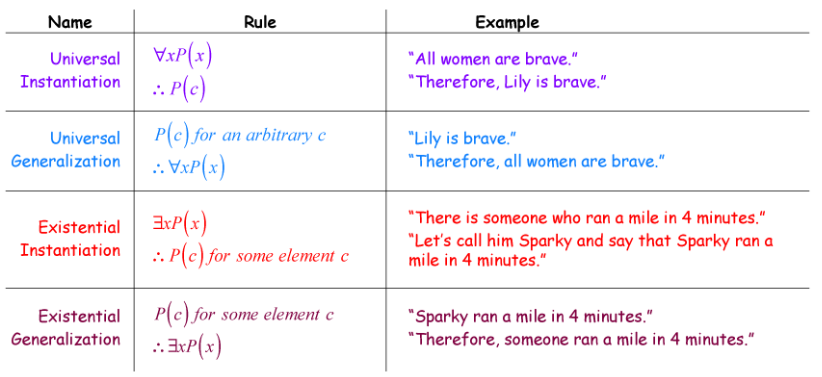
\includegraphics[height=6cm]{lecture18-fig1a.png}
   \end{center}

% Modify this part and the corresponding part in Lecture 17
% based on https://calcworkshop.com/logic/rules-inference/

\end{frame}

\begin{frame}[plain]{}

{\bf Example 18.5.} Translate the statement
\[ \forall x \left[ C(x)\vee \exists y \left( C(y)\wedge F(x,y)\right)\right] \]
into English, where $C(x)$ is ``$x$ has a computer,"
$F(x,y)$ is ``$x$ and $y$ are friends," and the domain
for both $x$ and $y$ consists of all students in your school.\pause
\medskip

{\bf Solution.} 
\begin{itemize}
 \item The statement says that for every student $x$ in your school, 
  $x$ has a computer or there
  is a student $y$ such that $y$ has a computer and $x$ and $y$ are friends. 
 \item In other words, every student
in your school has a computer or has a friend who has a computer. 
\end{itemize}

\end{frame}


\begin{frame}[plain]{ }

{\bf Example 18.6.} Translate the statement 
``\Blue{The sum of two positive integers is always positive}'' into a logical
expression. \pause

 \begin{itemize}[<+->]
  \item To translate this statement into a logical   expression, 
   we first rewrite it so that the implied
   quantifiers and a domain are shown:
     ``\Blue{For every two integers, if these integers are both positive,
then the sum of these integers is positive.}''
   \item Next, we introduce the variables $x$ and $y$ to obtain ``\Blue{For
all positive integers $x$ and $y$, $x+y$ is positive.}''
   \item Consequently, we can express this statement as
   \[ \Blue{\forall x\forall y [(x>0)\wedge (y>0) \rightarrow (x+y>0)] }\]
 where the domain for both variables consists of all integers.
 \item {\bf Remark}. If we restrict the domain to all positive integers only, then it becomes
 $\Blue{\forall x\forall y\, (x+y>0).}$
 \end{itemize}

\end{frame}

\begin{frame}[plain]{ }

{\bf Example 18.7.} 
Use quantifiers to express the statement 
"\Blue{There is a woman who has taken a flight on every airline in the world.}"
 \pause

 \begin{itemize}[<+->]
  \item Let $P(w,f)$ be "$w$ has taken $f$" and $Q(f,a)$ be "$f$ is a flight on $a$."
  \item We can express the statement as
  \[ \exists w \forall a  \exists f \left( P(w,f)\wedge Q(f,a)\right), 
  \]
  where the domains for $w$, $f$, and $a$, consist of all women,
  all airplane flights, and all airlines, respectively.
 \end{itemize}
 \vspace{.5in}
 

\end{frame}

\begin{frame}[plain]{}

 {\bf Practice 18.8.} Express the following system specification
  using predicates, quantifiers and logical connectives.
  
  \begin{quote}
   No directories in the file system can be opened and no files can be closed 
   when system errors have
   been detected.
  \end{quote}
  
  \vspace{1.5in}
  
\end{frame}

\end{document}


%%%%%%%%%%%%%%%%%%%%%%%%%%%%%%%%
 
\begin{frame}[plain]{Exercises}

  \begin{enumerate}
    \item If $R(x,y) = $ ``$x$ relies upon $y$,", express the following in English
  when the domain is all people.
    \begin{itemize}
      \item[(a)] $\forall\,x (\exists\,y\ R(x,y))$
      \item[(b)] $\exists\,y (\forall\,x \ R(x,y))$
      \item[(c)] $\exists\,x (\forall\,y\ R(x,y))$
      \item[(d)] $\forall\,y (\exists\,x\ R(x,y))$
      \item[(e)] $\forall\,x (\forall\,y\ R(x,y))$
    \end{itemize}
  
   \item Express the statement ``\Blue{If a person is female and is a parent, then this person is someone's
mother}'' as a logical expression involving predicates, quantifiers with a domain consisting of all
people, and logical connectives.%Rosen p62 Ex11
  \end{enumerate}

\end{frame}

\end{document}

%%%%%%%%%%%%%%%%%%%%%%%%%%%%%%

\begin{frame}[plain]{}

\begin{enumerate}
   \setcounter{enumi}{3}
   
  \item  Translate the statement ``\Blue{Every real number except zero has a multiplicative inverse.}'' 
   (A multiplicative inverse of a real number $x$ is a real number $y$ such that $xy = 1$.)
   %Rosen p61 Ex7
   
   \item Let $Q(x,y)$ be the statement $xy=0$. 
     If the domain for both variables consists of all integers, 
     what are the truth values of the following statements? 
     \begin{itemize}
       \item[(a)] $\forall x \forall y \ Q(x,y)$
       \item[(b)] $\exists x \forall y \ Q(x,y)$
       \item[(c)] Write a python code of determining the truth values in (a) and (b).
    \end{itemize}
     \item  Let $C(x,y)$ mean that student $x$ is enrolled in class $y$, where the domain of $x$ 
   consists of all students in AURAK and the domain for $y$ consists of all classes being given at
   AURAK. Express each of these statements by a simple English sentence.
   \begin{itemize}
    \item[(a)] $C(Ahmed, CSCI 211)$
    \item[(b)] $\exists x\,C(x, MATH 225)$
    \item[(c)] $\exists y\,C(Aisha, y)$
    \item[(d)] $\exists x\,\left( C(x, MATH 114)\wedge C(x, CSCI 211)\right)$
    \item[(e)] $\exists x\,\exists y\,\forall z \left[ (x\neq y)
     \wedge (C(x,z)\rightarrow C(y,z))\right]$
   \end{itemize}
 
 \end{enumerate}
 
 
 \end{frame}
 

%%%%%%%%%%%%%%%%%%%%%%%%%
